\section{Learning Curves}
If the learning model does not produce the expected results, most often either high bias or high variance is the cause.
A technique often used in practice is to compute the functions $J_{\text{train}}(\theta)$ and $J_{\text{val}}(\theta)$ by going to change the size of the training set:
\begin{center}
    \begin{tabular}{c}
        \\ 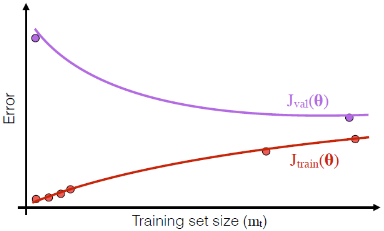
\includegraphics[width=0.5\textwidth]{images/LearningCurves1.png} \\ \\
    \end{tabular}
\end{center}
To understand how to use this type of curve let us analyze examples:
\begin{center}
    \begin{tabular}{c c c}
        \\ 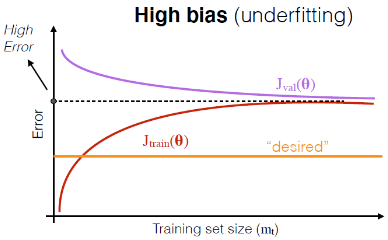
\includegraphics[width=0.5\textwidth]{images/LearningCurves2.png} & &
        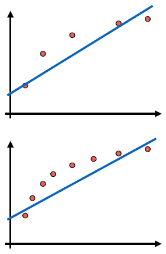
\includegraphics[width=0.2\textwidth]{images/LearningCurves3.png} \\ \\
    \end{tabular}
\end{center}
Here we are in a case of high bias (underfitting) where, increasing the size of the training set, does not help and errors are higher than expected.
\begin{center}
    \begin{tabular}{c c c}
        \\ 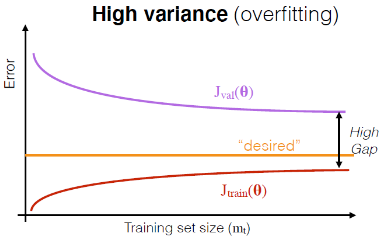
\includegraphics[width=0.5\textwidth]{images/LearningCurves4.png} & &
        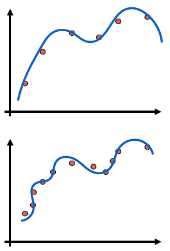
\includegraphics[width=0.2\textwidth]{images/LearningCurves5.png} \\ \\
    \end{tabular}
\end{center}
Here, on the other hand, we are in a case of high variance (overfitting) where the training error may be acceptable but the validation error is not, creating a large separation between the two curves. In cases like this increasing the size of the training set can help instead.

\newpage